% Supplementary Materials — compiled separately from the main manuscript.
% Figures are numbered S1–S6 and tables S1–S2 to match the back-matter declaration.
\documentclass[10pt]{article}
\usepackage[margin=2.5cm]{geometry}
\usepackage{graphicx}
\usepackage{float}
\usepackage{xcolor}
\usepackage{booktabs}
\usepackage{tabularx}
\usepackage{amsmath}
\usepackage{amssymb}
\usepackage[font=small,labelfont=bf]{caption}
\usepackage{hyperref}

\renewcommand{\thetable}{S\arabic{table}}
\renewcommand{\thefigure}{S\arabic{figure}}
\renewcommand{\thesection}{S\arabic{section}}
\newcolumntype{C}{>{\centering\arraybackslash}X}

\title{Supplementary Materials for\\\textbf{WaveletMask: Wavelet-Domain Mask-Guided Degradation Detection for Old Film Restoration}}
\author{}
\date{}

\begin{document}
\maketitle

\noindent This document provides the supplementary figures and tables referenced from the main manuscript: complete diagnostic example grids (Figures~\ref{fig:s1}--\ref{fig:s3}), the expert-level subjective quality evaluation (Tables~\ref{tab:s1}--\ref{tab:s2} and Figure~\ref{fig:s4}), the spatial error-map analysis (Figure~\ref{fig:s5}), and the probe visualization overview (Figure~\ref{fig:s6}).

\section{Complete Diagnostic Example Grids}

Figures~\ref{fig:s1}--\ref{fig:s3} provide the complete example grids for the three detector diagnostic probes reported in Appendix~C of the main manuscript.

\begin{figure}[H]
\centering
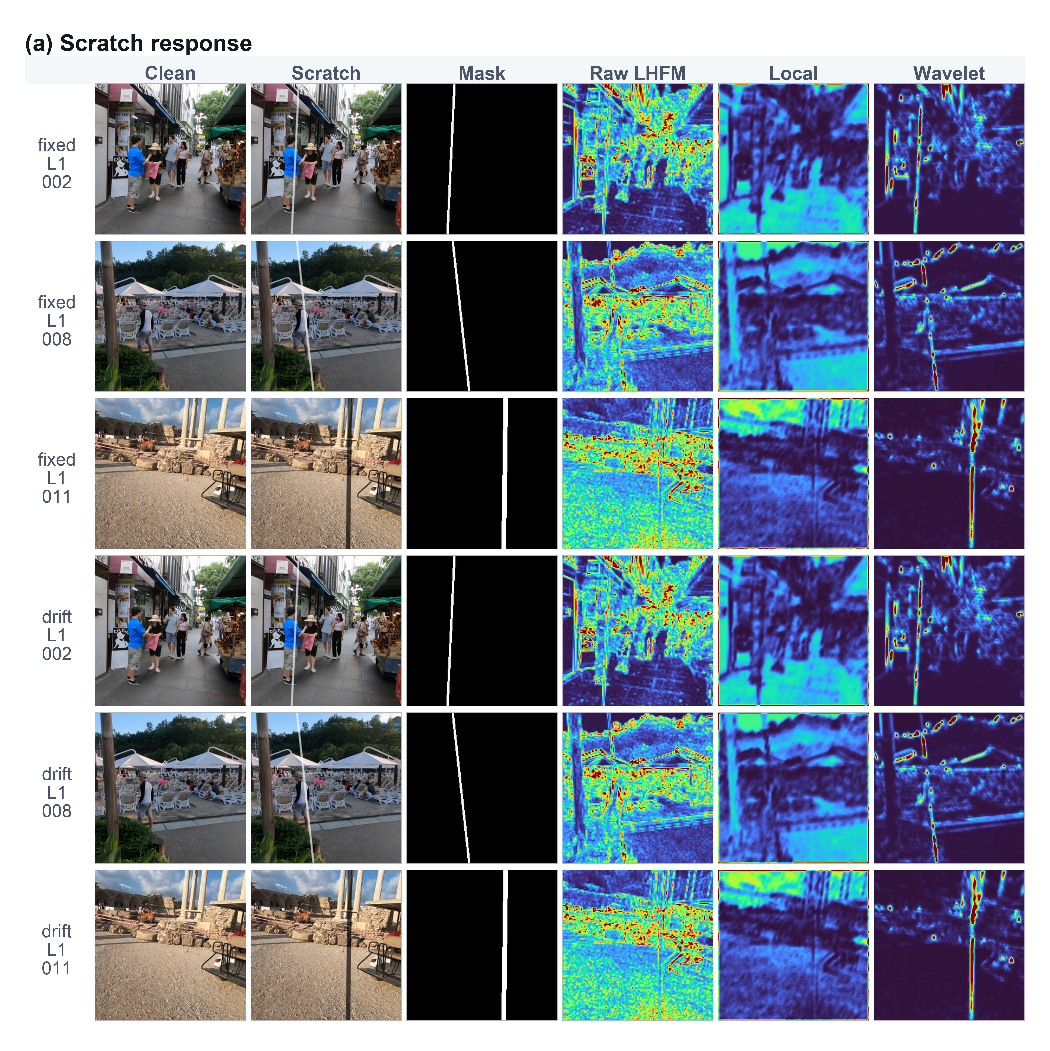
\includegraphics[width=0.75\textwidth]{figures/FigureS1_PersistentScratchDiagnostic.pdf}
\caption{Complete persistent-scratch diagnostic examples. Each row compares clean frames, injected scratches, scratch masks, raw LHFM responses, learned local masks, and fused wavelet masks.\label{fig:s1}}
\end{figure}

\begin{figure}[H]
\centering
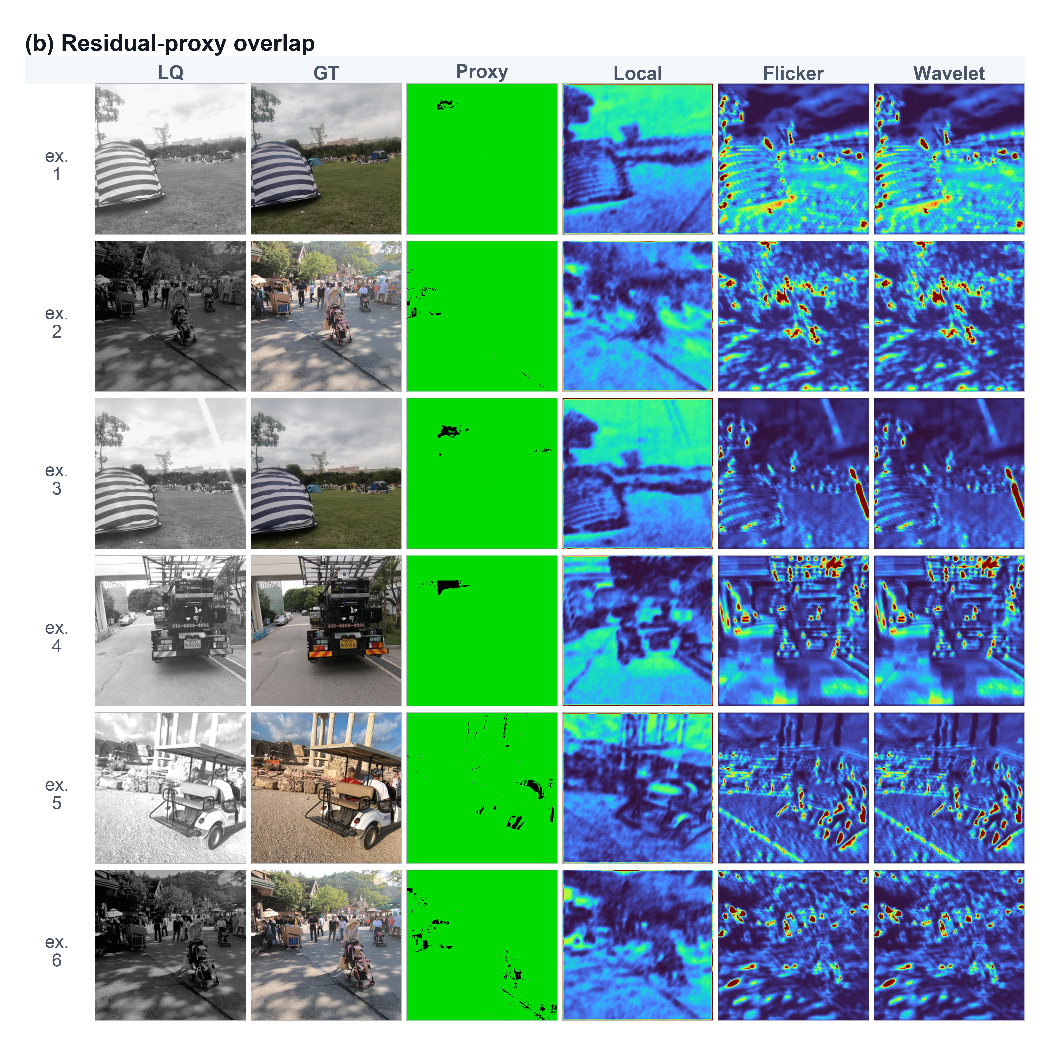
\includegraphics[width=0.75\textwidth]{figures/FigureS2_MaskInterpretabilityDiagnostic.pdf}
\caption{Complete residual-proxy overlap examples. Each row compares paired input--ground-truth residual proxies with learned local, flicker, and wavelet mask responses.\label{fig:s2}}
\end{figure}

\begin{figure}[H]
\centering
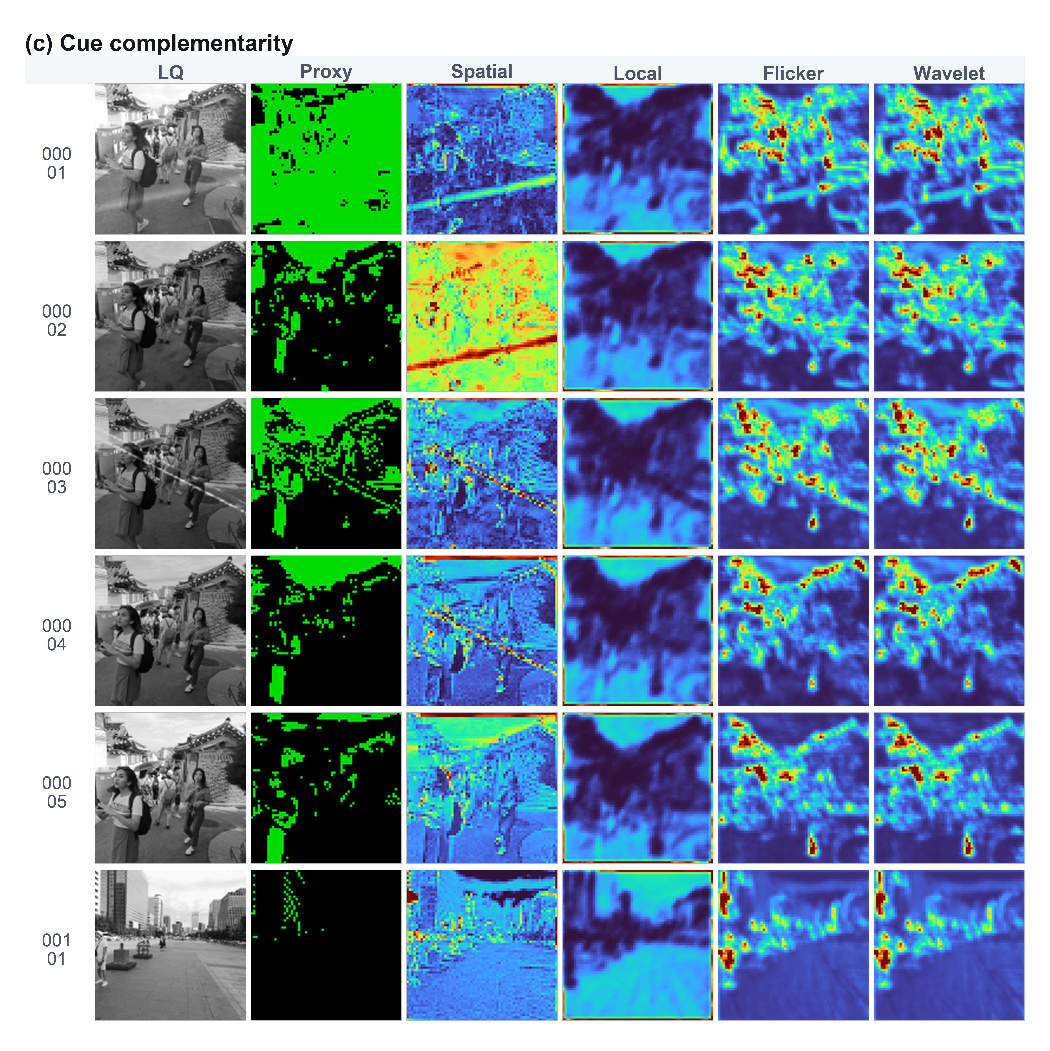
\includegraphics[width=0.75\textwidth]{figures/FigureS3_CueComplementarityDiagnostic.pdf}
\caption{Complete cue-complementarity examples. Each row compares the flow-aligned spatial indicator with the local, flicker, and wavelet responses on the same frame.\label{fig:s3}}
\end{figure}

\section{Expert-Level Subjective Quality Evaluation}

To complement the content-sensitive no-reference metrics on the SRWOV real-world split, we conducted an internal expert visual-quality scoring with 34 domain-specialized internal raters. Each rater ranked four methods (WaveletMask, MambaOFR, RRTN, RTN) on 14 real old-film clips across three perceptual dimensions---degradation removal, style preservation, and temporal consistency---plus overall best visual experience. This internal panel provides an expert-level visual assessment while collecting only method-preference scores for the restored images. Presentation order was randomized per rater and per clip; raters were blind to method identity.

\begin{table}[H]
\caption{Overall preference in the internal expert-level subjective evaluation (34 internal expert raters $\times$ 14 clips = 476 responses). Each response selects the method with the best visual experience. The best result is in \textcolor{red}{red}.\label{tab:s1}}
\begin{tabularx}{\textwidth}{lCC}
\toprule
\textbf{Method} & \textbf{Votes} & \textbf{Percent} \\
\midrule
\textbf{WaveletMask} & \textcolor{red}{215} & \textcolor{red}{45.17\%} \\
MambaOFR & 114 & 23.95\% \\
RRTN & 86 & 18.07\% \\
RTN & 61 & 12.82\% \\
\bottomrule
\end{tabularx}
\end{table}

\begin{table}[H]
\caption{Rank-1 counts by perceptual dimension (476 responses per dimension). The method receiving the most first-place votes per dimension is in \textcolor{red}{red}.\label{tab:s2}}
\begin{tabularx}{\textwidth}{lCCCC}
\toprule
\textbf{Dimension} & \textbf{WaveletMask} & \textbf{MambaOFR} & \textbf{RRTN} & \textbf{RTN} \\
\midrule
Degradation removal & \textcolor{red}{264 (55.5\%)} & 112 (23.5\%) & 70 (14.7\%) & 30 (6.3\%) \\
Style preservation & \textcolor{red}{247 (51.9\%)} & 132 (27.7\%) & 67 (14.1\%) & 30 (6.3\%) \\
Temporal consistency & \textcolor{red}{273 (57.4\%)} & 107 (22.5\%) & 69 (14.5\%) & 27 (5.7\%) \\
\bottomrule
\end{tabularx}
\end{table}

Table~\ref{tab:s1} shows that WaveletMask receives 45.17\% overall preference, outperforming the second-ranked MambaOFR (23.95\%) by nearly $2\times$ and RTN by 3.5$\times$. Table~\ref{tab:s2} shows the same pattern across all three perceptual dimensions: WaveletMask ranks first in degradation removal (55.5\%), style preservation (51.9\%), and temporal consistency (57.4\%). This is because LHFM suppresses local structural defects while GFM stabilizes low-frequency brightness fluctuation across frames. These preferences are statistically significant: the overall distribution deviates strongly from the uniform chance distribution ($\chi^2(3)=115.1$, $p=8.9\times10^{-25}$), and the WaveletMask share of 45.17\% (Wilson 95\% CI $[40.8\%, 49.7\%]$) lies significantly above the 25\% chance level of the four-method ranking (one-sided exact binomial test, $p=1.1\times10^{-21}$). The per-dimension rank-1 distributions are likewise significantly non-uniform (all $\chi^2(3)\ge228.4$, $p<10^{-48}$). These tests treat the 476 votes as independent draws and do not model rater-level clustering, because only aggregated vote exports are available. Figure~\ref{fig:s4} summarizes the overall preference distribution and the per-dimension ranking statistics.

\begin{figure}[H]
\centering
\begin{minipage}{0.45\textwidth}
\centering
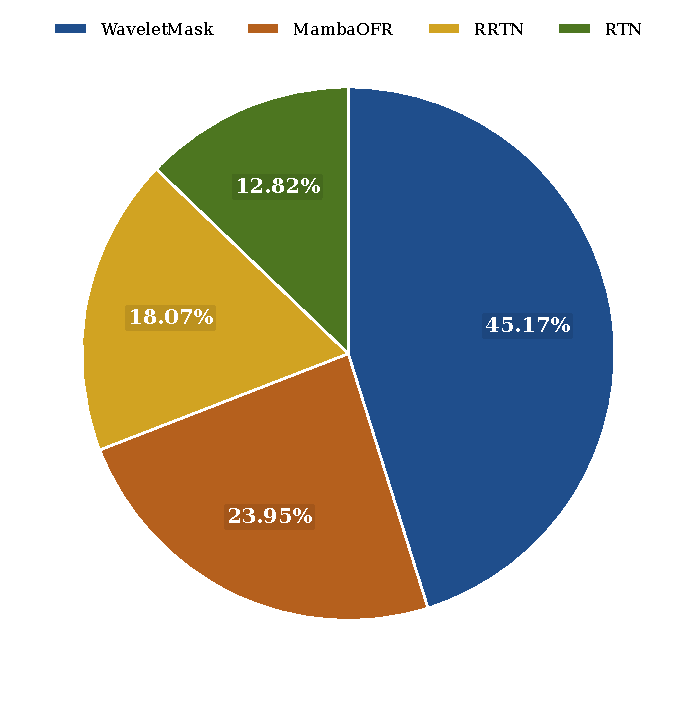
\includegraphics[width=\textwidth]{figures/FigureS4a_UserStudyPreference.pdf}
\par\smallskip
(a)
\end{minipage}\hfill
\begin{minipage}{0.45\textwidth}
\centering
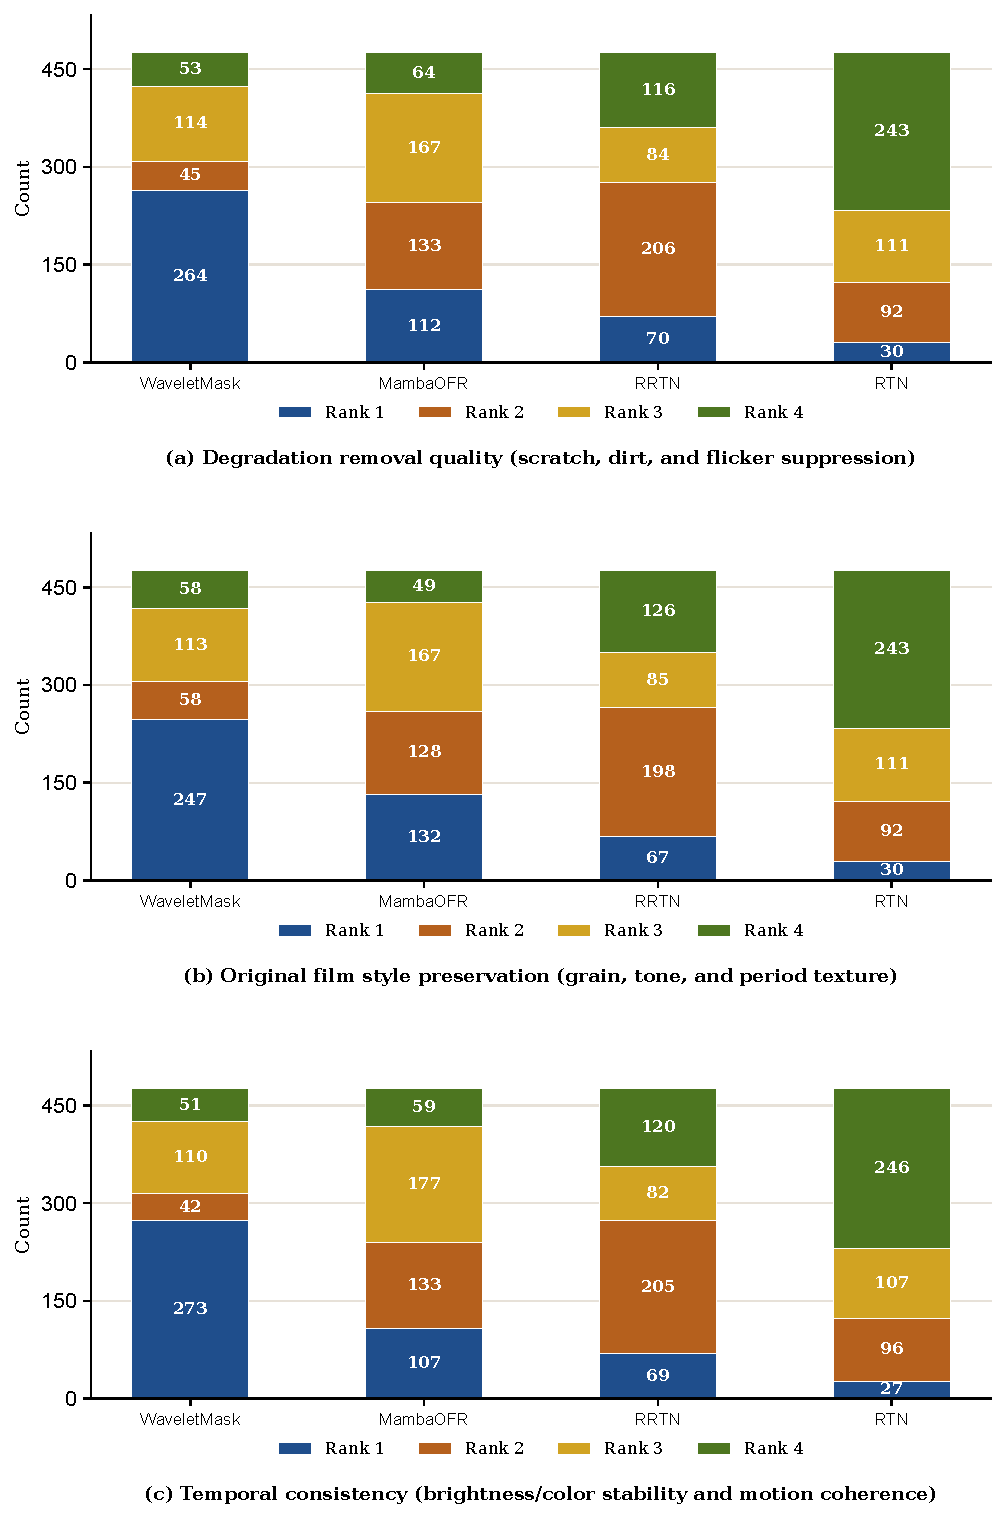
\includegraphics[width=\textwidth]{figures/FigureS4b_UserStudyRanking.pdf}
\par\smallskip
(b)
\end{minipage}
\caption{Internal expert-level subjective evaluation results. (a) Overall preference distribution from the 34-rater internal study on 14 real old-film clips. (b) Rank-1 counts across three perceptual dimensions; WaveletMask achieves the highest first-place count in all dimensions.\label{fig:s4}}
\end{figure}

\section{Spatial Error-Map Analysis}

Figure~\ref{fig:s5} compares absolute error maps between the RTN and WaveletMask on selected synthetic frames with ground truth. The selected frames satisfy the recorded filter conditions used to generate the figure, including a PSNR gain above 1~dB, non-decreasing SSIM, and an improved-pixel ratio above 55\%. The red improvement maps identify pixels where WaveletMask has lower absolute error than the baseline, showing that the gain is spatially concentrated around damaged regions in these examples.

\begin{figure}[H]
\centering
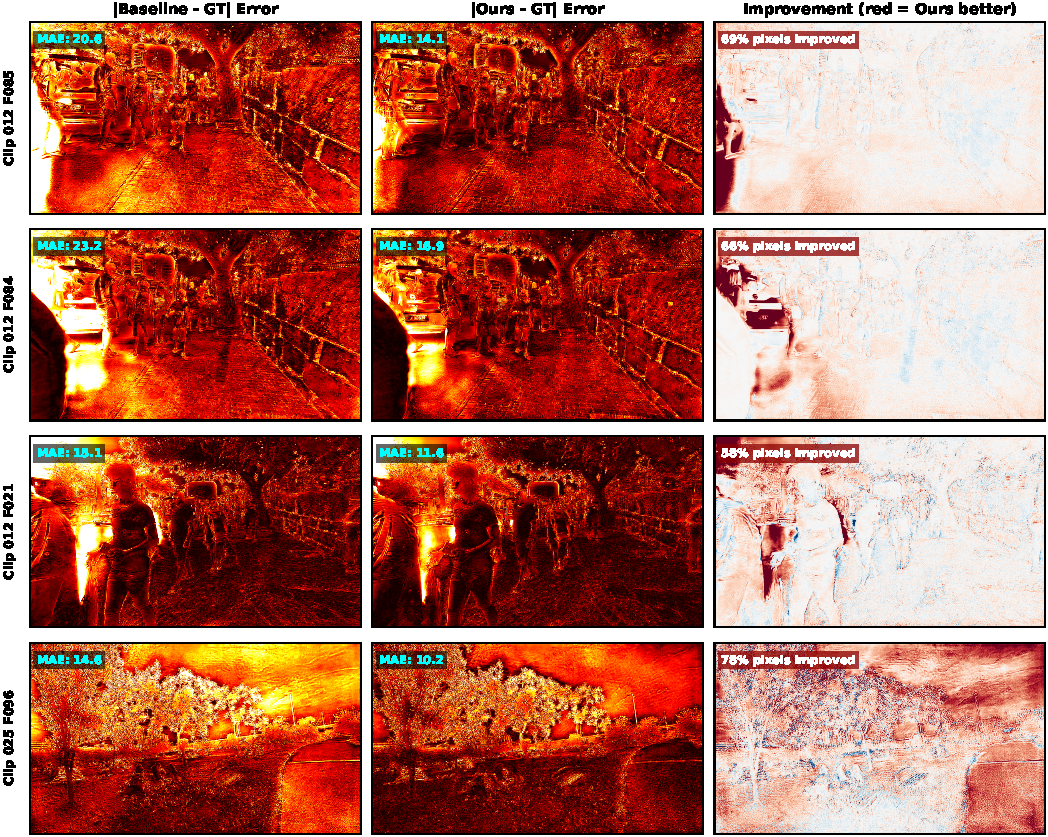
\includegraphics[width=\textwidth]{figures/FigureS5_ErrorMap.pdf}
\caption{Error-map comparison between the RTN and WaveletMask on selected SRWOV synthetic frames. The first two columns report absolute error with respect to GT; the third column marks pixels where WaveletMask has lower error in red.\label{fig:s5}}
\end{figure}

\section{Probe Visualization Overview}

Figure~\ref{fig:s6} summarizes representative visual examples for the three detector probes; the persistent-scratch examples use single-frame ($L=1$) injections and therefore highlight detector-response patterns, while the persistence-length trend is quantified in Appendix~C of the main manuscript.

\begin{figure}[H]
\centering
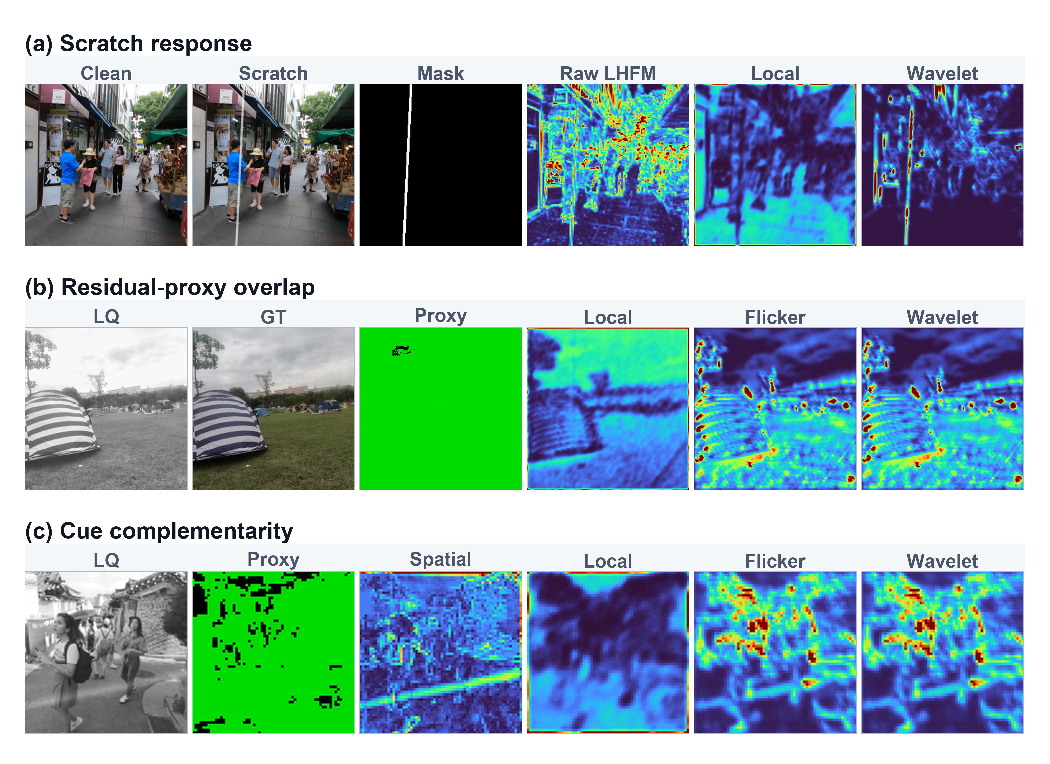
\includegraphics[width=\textwidth]{figures/FigureS6_DiagnosticVisualization.pdf}
\caption{Visualization for the wavelet-mask probes. (a) Persistent-scratch examples compare clean frames, injected scratches, scratch masks, raw LHFM responses, learned local masks, and fused wavelet masks. (b) Residual-proxy examples compare paired input--ground-truth residual proxies with learned local, flicker, and wavelet mask responses. (c) Cue-complementarity examples compare the flow-aligned spatial indicator with the local, flicker, and wavelet responses on the same frame.\label{fig:s6}}
\end{figure}

\end{document}
